%&pdflatex
\documentclass[a4paper,12pt]{article}
\usepackage{amssymb, amsmath}
\usepackage[utf8]{inputenc}
\usepackage[T2A,T1]{fontenc}
\usepackage[english,russian]{babel}
\usepackage{csquotes}
% \IfFileExists{literat.sty}{\usepackage{literat}}{}

\usepackage{fullpage}
\usepackage{indentfirst}
\usepackage[font=small,labelfont=bf,labelsep=period]{caption}

\usepackage{wrapfig}
\usepackage{graphicx}
\usepackage{media9}

\newcommand{\Kn}{\mathrm{Kn}}
\newcommand{\dd}{\mathrm{d}}
\newcommand{\pder}[2][]{\frac{\partial#1}{\partial#2}}
\newcommand{\pderdual}[2][]{\frac{\partial^2#1}{\partial#2^2}}
\newcommand{\pderder}[3][]{\frac{\partial^2#1}{\partial#2\partial#3}}
\newcommand{\Pder}[2][]{\partial#1/\partial#2}

\usepackage[
    pdfauthor={Rogozin Oleg},
    pdftitle={Couette Flow and Heat Transfer between Two Parallel Plates},
    colorlinks,pdftex, unicode]{hyperref}

\usepackage[
    backend=biber,
    style=alphabetic,
    language=british,
    sorting=nyt,
    url=false,
    eprint=false,
    pagetracker,
    firstinits]{biblatex}
\bibliography{couette_heat}

\usepackage[toc]{appendix}
\renewcommand{\appendixtocname}{Приложения}
\renewcommand{\appendixpagename}{Приложения}
\renewcommand{\appendixname}{Приложениe}

\title{Течение Куэтта и перенос тепла между двумя параллельными пластинами}
\author{Рогозин Олег}

\begin{document}
\maketitle
\tableofcontents

\section{Введение}

Одномерные задачи течения Куэтта и переноса тепла между двумя параллельными пластинами являются наиболее простыми,
но основополагающими в динамике разреженного газа. В работе изучаются линейные приближения задач,
которые соответствуют малым градиентам макропараметров. В такой постановке они хорошо изучены
для всего диапазона чисел Кнудсена, и при этом подробно табулированы с высокой точностью.
Целью работы является верификация проекционного метода решения кинетического уравнения Больцмана
на основе точного решения линеаризованного приближения.

\section{Постановка задачи}

Рассмотрим одноатомный идеальный газ между двумя бесконечными параллельными пластинами с полным диффузным отражением.
Ось абсцисс направлена параллельно пластинам, расстояние между которыми равно \(L\).
В качестве молекулярного потенциала взаимодействия выберем модель твердых сфер.

Течение Куэтта образуется при относительном движении пластин друг относительно друга с продольной скоростью
вдоль оси абсцисс, при этом температура стенок одинакова и остаётся постоянной.
Задача переноса тепла ставится для фиксированного отношения температур покоящихся пластин.

\section{Основные уравнения}

В работе будем иметь дело с безразмерными величинами, такими, что макроскопические величины будут
иметь следующий вид: давление \(pp^{(0)}\), температура \(TT^{(0)}\), плотность \(\rho p^{(0)}/RT^{(0)}\)
скорость \(v_i(2RT^{(0)})^{1/2}\) и тепловой поток \(q_ip^{(0)}(2RT^{(0)})^{1/2}\),
где \(R = k_B/m\) "--- удельная газовая постоянная,
равная отношению постоянной Больцмана \(k_B\) к молекулярной массе \(m\),
а \(T^{(0)}\) "--- средняя температура пластин.
За единицу длины примем расстояние между пластинами \(L\).
Расчётная область, представленная на рис.~\ref{fig:geometry} серым фоном,
лежит в диапазоне \(0 \le y\le 1/2\) вследствие антисимметрии задачи.
Температура и скорость верхней пластины (\(y=1/2\)) равны \((1+\Delta T/2)T^{(0)}\)
и \((U/2)(2RT^{(0)})^{1/2}\), соответственно.

\begin{figure}[ht]
    \centering
    \includegraphics{tikz/geometry}
    \caption{Геометрия задачи}
    \label{fig:geometry}
\end{figure}

Стационарное уравнение Больцмана в безразмерных переменных принимает следующий вид:
\begin{equation}\label{eq:Boltzmann}
    \zeta_i\pder[f]{x_i} = \frac1k J(f,f),
\end{equation}
в котором интеграл столкновений
\begin{equation}
    J(f,g) = \frac12 \int (f'g'_* + f'_*g' - fg_* - f_*g) B
    \dd \Omega(\boldsymbol{\alpha}) \boldsymbol{\dd \zeta_*},
\end{equation}
берётся от функции распределения \(f(x_i,\zeta_i)(2p^{(0)})/(2RT^{(0)})^{5/2}\), представленной
в пространстве \((x_iL, \zeta_i(2RT^{(0)})^{1/2})\).
\(\dd \Omega(\boldsymbol{\alpha})\) "--- элемент телесного угла в направлении единичного вектора \(\alpha_i\),
определяющего направление разлётных скоростей:
\[
    \zeta'_i = \zeta_i + \alpha_i\alpha_j(\zeta_{j*}-\zeta_j), \quad
    \zeta'_{i*} = \zeta_{i*} - \alpha_i\alpha_j(\zeta_{j*}-\zeta_j).
\]
Функция \(B\) определяется законом межмолекулярного взаимодействия.
В частном случае модели твёрдых сфер
\begin{equation}
    B = \frac{|\alpha_i(\zeta_{i*}-\zeta_i)|}{4\sqrt{2\pi}}.
\end{equation}
В уравнении~\eqref{eq:Boltzmann} используется модифицированное число Кнудсена
\begin{equation}
    k = \frac{\sqrt\pi}2 \Kn = \frac{\sqrt\pi\ell_0}{2L} =
    \frac{mRT^{(0)}}{2\sqrt{2\pi} d_m^2p^{(0)}L},
\end{equation}
где \(\ell_0\) "--- средняя длина свободного пробега, определяемая радиусом межмолекулярного
взаимодействия \(d_m\) (для модели твёрдых сфер совпадает с диаметром молекулы).

Макропараметры газа вычиляются с помощью интегрирования функции распределения по формулам:
\begin{alignat*}{2}
    \rho &= \int f \boldsymbol{\dd\zeta}, \\
    v_i &= \frac1{\rho} \int \zeta_i f \boldsymbol{\dd\zeta}, \\
    T &= \frac{2}{3\rho}\int(\zeta_i-v_i)^2 f \boldsymbol{\dd\zeta}, \\
    p_{ij} &= 2 \int(\zeta_i-v_i)(\zeta_j-v_j) f \boldsymbol{\dd\zeta},
        \quad p \equiv p_{ii}/3 = \rho T, \\
    q_i &= \int(\zeta_i-v_i)(\zeta_j-v_j)^2 f \boldsymbol{\dd\zeta}.
\end{alignat*}

\section{Методика численного решения уравнения Больцмана}

Кинетическое уравнение Больцмана решалось симметричным методом расщепления на уравнение переноса
\[ \frac{\partial\hat{f}}{\partial\hat{t}} + \zeta_i\frac{\partial\hat{f}}{\partial x_i} = 0, \]
для которого использовалась консервативная TVD схема с ограничителем третьего порядка аппроксимации,
и уравнение релаксации
\[ \frac{\partial\hat{f}}{\partial\hat{t}} = \hat{J}(\hat{f},\hat{f}), \]
которое в свою очередь решалось проекционным методом.

В качестве дискретного пространства скоростей использовался шар радиусом \(4.3\nu_0\)\footnote
{
    4.3 тепловых скорости достаточно, чтобы обеспечить точность 0.01\% совпадения
    первых тринадцати моментов функции распределения (малой величины) с соответствующими разностными аналогами.
},
равномерно заполненный узлами так, что на радиусе помещалось 16 точек.
Одномерное координатное пространство состояло как минимум из 30 одинаковых кубических ячеек,
при условии что их размер не превышал единицы.

Для взятия интеграла столкновений применялись сетки Коробова размером от 0.1 до 1 млн. точек.
Стационарные значения макропараметров усредненялись на последних 500 временных итераций,
что обеспечивало точность не ниже 0.1\%.

Для ускорения расчётов в качестве начальной функции распределения выбиралось тринадцатимоментное приближение Грэда
\[
    \hat{f}_{G13} = \frac{\hat\rho}{(\pi\hat T)^{3/2}}\exp\left(-\frac{c_i^2}{\hat T}\right)
    \left( 1+\frac{\hat p_{ij}c_ic_j}{\hat p\hat T} + \frac4{5}\frac{\hat q_ic_i}{\hat p\hat T}\left(\frac{c_i^2}{\hat T}-\frac5{2}\right) \right),
    \quad c_i = \zeta_i - \hat v_i
\]
с соответствующими точному решению профилями макропараметров.

В задаче Куэтта относительная скорость пластин равнялась \(\hat{U}=0.01\),
и такое же значение отношения температур \(\hat{T}_1/\hat{T}_2\) использовалось в задаче теплопереноса.
Этого достаточно, чтобы обеспечить линейность задачи с точностью порядка 0.01\%.

\section{Результаты}

\subsection{Течение Куэтта}

Для задачи Куэтта сравнивались зависимости сдвигового напряжения (рис.~\ref{fig:couette:shear}),
потоков массы (рис.~\ref{fig:couette:flow}) и тепла (рис.~\ref{fig:couette:qflow})
через половину сечения от числа Кнудсена.

В рамках линейной теории для бесстолкновительного газа
\[ \frac{\hat{p}_{xy}}{\hat{U}} = -\frac1{\sqrt{\pi}}, \]
а при небольших \(\Kn\) справедливо асимптотическое решение\footnote
{ Получается при решении уравнения Больцмана методом Грэда"--~Гильберта~\cite{Sone2007}: разложение по малому параметру \(\Kn\). }
\[ \frac{\hat{p}_{xy}}{\hat{U}} = \frac{2\hat{\mu}\Kn}{1-\sqrt{\pi}k_0\Kn}. \]
Коэффициенты вязкости \(\hat{\mu}\) и скольжения \(k_0\) для модели твёрдых сфер равны~\cite{Sone2007}
\[ \hat{\mu} = 0.562773, \; k_0 = -1.2540. \]
Отбросив знаменатель, получим гидродинамическое решение \(\hat{p}_{xy} = 2\hat{\mu}\Kn\hat{U}\).
Численные значения точного решения табулированы в~\cite{Sone1990}.

Кроме того, для сравнения представлены некоторые результаты
решения модельного кинетического уравнения БКВ (Больцмана"--~Крука"--~Веландера).
Несмотря на хорошое совпадение модельного решения с точным для значения сдвигового напряжения,
метод БКВ даёт значительную погрешность для потоков массы и тепла~\cite{Sone1990},
поэтому нигде не приводятся соответствующих табличных значений.

\begin{figure}
    \centering
    \includegraphics{couette/graph.pdf}
    \caption{Зависимость сдвигового напряжения от числа Кнудсена}\label{fig:couette:shear}
\end{figure}

\begin{figure}
    \centering
    \includegraphics{couette/flow.pdf}
    \caption{Зависимость потока массы через половину сечения от числа Кнудсена}\label{fig:couette:flow}
\end{figure}

\begin{figure}
    \centering
    \includegraphics{couette/qflow.pdf}
    \caption{Зависимость потока тепла через половину сечения от числа Кнудсена}\label{fig:couette:qflow}
\end{figure}

На рис.~\ref{fig:couette:shear} наблюдается хорошое совпадение результатов.
Однако для бесстолкновительного газа заметно превышение \(\hat{p}_{xy}\) на 0.61\%,
что может быть обусловлено только ошибкой дискретной аппроксимации функции распределения по скоростному пространству.
При интерполяции полученной кривой на интервале \(\Kn\in[0,0.2]\) асимптотическим решением
можно произвести подбор параметров нелинейным методом наименьших квадратов.
С его помощью в области континуального описания газа определяется оклонение
от коэффициентов вязкости (\(+0.83\%\)) и скольжения (\(-1.2\%\)).
Если все полученные значения нормировать на точное значение для бесстолкновительного газа (разделить на 1.0061),
то погрешность в коэффициенте вязкости снижается до \(+0.22\%\), что является уже приемлимым результатом.

На рис.~\ref{fig:couette:flow},~\ref{fig:couette:qflow} для сильно разреженного газа наблюдаются
значительные отклонения, природа которых пока не определена.

\subsection{Перенос тепла}

Для задачи переноса тепла проанализируем зависимость теплового потока \(q\) от числа Кнудсена (рис.~\ref{fig:heat}).

В рамках линейной теории для бесстолкновительного газа
\[ \frac{\hat{q}_x}{\hat{T}_1-\hat{T}_2} = -\frac1{\sqrt{\pi}}, \]
а при небольших \(\Kn\) справедливо асимптотическое решение
\[ \frac{\hat{q}_x}{\hat{T}_1-\hat{T}_2} = -\frac{\hat{\lambda}\Kn}{1+\sqrt{\pi}d_1\Kn}. \]
Коэффициенты теплопроводности \(\hat{\lambda}\) и скачка температуры на стенке \(d_1\) для модели твёрдых сфер равны~\cite{Sone2007}
\[ \hat{\lambda} = 2.129475, \; d_1 = 2.4001. \]
Отбросив знаменатель, получим гидродинамическое решение \(\hat{q}_x = -\hat{\lambda}\Kn(\hat{T}_1-\hat{T}_2)\).
Численные значения точного решения табулированы в~\cite{Sone2007}.

\begin{figure}
    \centering
    \includegraphics{heat/graph.pdf}
    \caption{Зависимость теплового потока от числа Кнудсена}\label{fig:heat}
\end{figure}

Как и в задаче о течении Куэтта, на рис.~\ref{fig:heat} видна хорошая сходимость к точному решению,
однако одновременно наблюдаются те же проблемы: завышение значений теплопотока на \(0.63\)\%
для бесстолкновительного газа и значительная ошибка в коэффициенте теплопроводности (\(+2.2\%\)).
По всей видимости, последняя объясняется неточной аппроксимацией угла разлёта сталкивающихся молекул,
в частности, существованием минимально разрешимого угла.

\subsection{Исследование погрешности}

Логичным представляется исследование зависимости указанных погрешностей от числа интерполирующих узлов
скоростного пространства. Будем анализировать ошибки аппроксимации задачи переноса тепла.
Для этого коэффициент теплопроводности вычислялся локально в точке \(x_0=\hat L/2\) по формуле
\[ \hat{q_x}(x_0) = -\hat{\lambda}\frac{\dd\hat T}{\dd x}\bigg|_{x=x_0}. \]

Соответствующие графики в логарифмическом масштабе представлены на рис.~\ref{fig:error}.
Наклон прямых говорит примерно о квадратичной зависимости:
\[ \varepsilon \propto R_\Omega^{-2} \propto V_\Omega^{-2/3}, \]
где \(R_\Omega\) "--- число узлов на радиусе скоростной сетки, \(V_\Omega\) "--- её объём.

При \(R_\Omega = 40\) точность вычисления теплового потока повышается до \(0.1\%\),
а коэффициента теплопроводности только до \(0.5\%\).
Отклонение точки \(R_\Omega = 40\) для \(\lambda\) объясняется прямой по всей видимости

\begin{figure}
    \centering
    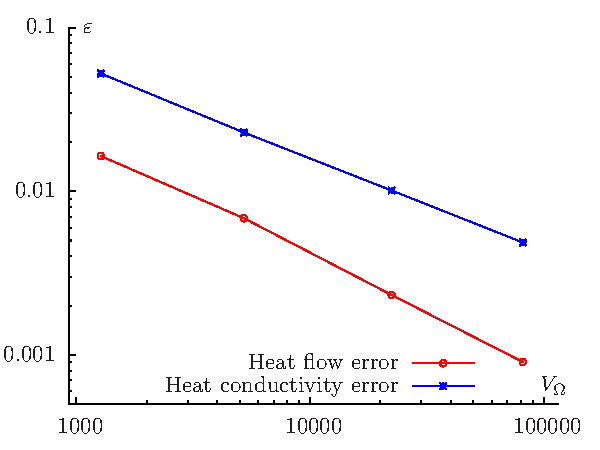
\includegraphics{error/error.pdf}
    \caption{
        Зависимость от числа узлов на радиусе скоростной сетки погрешностей вычисления
        теплопотока для бесстолкновительного газа и коэффициента теплопроводности для слаборазреженного газа
    }\label{fig:error}
\end{figure}

\section{Заключение}

Показана удовлетворительная сходимость численного решения уравнения Больцмана проекционным методом
простейших одномерных линейных задач: течения Куэтта и переноса тепла, --- к эталонным на основе
линеаризованного уравнения.

Выявлены две проблемы. Во-первых, плохая сходимость погрешности аппроксимации теплового потока по отношению к
объёму используемой памяти. Возможным решением является корректировка всех значений макропараметров
по их отклонению в бесстолкновительном режиме при используемом \(R_\Omega\) от некоторого большего \(R_\Omega\),
при котором результаты можно считать достоверными.

Во-вторых, существенна погрешность в определении коэффициентов вязкости и особенно теплопроводности.
По всей видимости, качественно улучшить аппроксимацию межмолекулярного потенциала позволит лишь использование
более чем двухточечного проекционного метода, который обеспечит точное значение угла разлёта.

\appendix
\appendixpage

\section{Функции Абрамовица}\label{sec:Abramowitz}

Семейство функций Абрамовица~\cite{Cercignani2000} имеют следующий вид:
\begin{equation}\label{eq:Abramowitz}
    \mathcal{T}_n(s) = \int_0^\infty t^n \exp\left(-t^2-\frac{s}{t}\right) \dd t,
    \quad s\ge0, \quad n \in \mathbb{Z}.
\end{equation}
Из очевидного соотношения \(\dd \mathcal{T}_n/\dd x = -\mathcal{T}_{n-1}\) следует, что
\[
    \lim_{s\to0} \frac{\dd^{n+1} \mathcal{T}_n(s)}{\dd s^{n+1}} = \infty.
\]
Таким образом, функции \(\mathcal{T}_n(s)\) неаналитичны ввиду особенности в точке \(x=0\),
поэтому не могут быть разложены непосредственно в ряд Тейлора.

Найдём, тем не менее, приближение \(\mathcal{T}_0(s)\) при малых \(s\):\footnote{
    В монографии К.~Черчиньяни <<Динамика разреженного газа>>~(2000)~\cite{Cercignani2000}
    допущена ошибка в форм.~(2.4.19).
}
\begin{gather}
    \mathcal{T}_0(s) = \int_0^1 \left(e^{-t^2}-1\right) e^{-\frac{s}{t}} \dd{t}
        + \int_1^\infty e^{-t^2} e^{-\frac{s}{t}} \dd{t}
        + \int_0^1 e^{-\frac{s}{t}} \dd{t} \notag\\
    = \int_0^1 \left(e^{-t^2}-1\right) \sum_{k=0}^2 \frac{(-s)^k}{k!t^k} \dd{t}
        + \int_1^\infty e^{-t^2} \sum_{k=0}^2 \frac{(-s)^k}{k!t^k} \dd{t}
        + s\int_s^\infty \frac{e^{-t}}{t^2} \dd{t} + o(s^2) \notag\\
    = \left(\frac{\sqrt\pi}2-1\right)
        + \frac{\gamma}2 s
        + (1-\sqrt\pi) \frac{s^2}2
        + e^{-s} - \int_s^\infty\frac{e^{-t}}{t} \dd{t} + o(s^2)  \notag\\
    = \frac{\sqrt\pi}2
        + s\ln{s} + \left(\frac{3\gamma}2 - 1\right) s
        - \sqrt\pi\frac{s^2}2 + o(s^2) \label{eq:Abramowitz0}
\end{gather}
Здесь используется интегральная показательная функция
\begin{equation}\label{eq:exp_integral}
    \mathrm{Ei}(s) = -\int_{-s}^\infty \frac{e^{-t}}{t} \dd{t}
        = \gamma + \ln|s| + \sum_{k=1}^{\infty} \frac{s^k}{kk!},
\end{equation}
где \(\gamma\) "--- постоянная Эйлера"--~Маскерони:
\begin{equation}\label{eq:euler-masceroni}
    \gamma = -\int_0^\infty e^{-t}\ln{t} \dd{t}
        = \int_0^1 \frac{1-e^{-t}}{t} \dd{t} - \int_1^\infty \frac{e^{-t}}{t} \dd{t}.
\end{equation}

Дальнейшее разложение в ряд приводит к следующим рекуррентным
соотношениям~\cite{Abramowitz1953,Abramowitz1972}:\footnote{
    В справочнике по специальным функциям М.~Абрамовица, И.~Стиган~(1979)~\cite{Abramowitz1972}
    см. форм.~(27.5.4).
}
\begin{gather}\label{eq:Abramowitz1-full}
    \mathcal{T}_1(s) = \frac12\sum_{k=0}^\infty ( a_k \ln{k} + b_k ) s^k, \\
    \begin{alignedat}{2}
        a_k &= \frac{-2a_{k-2}}{k(k-1)(k-2)}, &\quad b_k &= \frac{-2b_{k-2} - (3k^2-6k+2)a_k}{k(k-1)(k-2)}, \quad k>2, \\
        a_0 &= a_1 = 0, \quad a_2 = -1, &\quad b_0 &= 1, \quad b_1 = -\sqrt\pi, \quad b_2 = \frac32(1-\gamma).
    \end{alignedat} \notag
\end{gather}
В частности, дифференцируя~\eqref{eq:Abramowitz0}, получаем
\begin{equation}\label{eq:Abramowitz-1}
    \mathcal{T}_{-1}(s) = - \ln{s} - \frac{3\gamma}2 + \sqrt\pi s + O(s^2\ln{s}).
\end{equation}

\section{Численное решение задачи Куэтта для модели БКВ}\label{sec:numerical_bkw}

Решение задачи Куэтта в рамках линеаризованного уравнения БКВ
сводится к решению уравнения~\eqref{eq:bkw_g_equation}.
Основная сложность решения неоднородного интегрального уравнения Фредгольма второго рода для \(g(y)\)
"--- это логарифмические особенности ядра и первой производной свободного члена
[см.~\eqref{eq:Abramowitz0} и~\eqref{eq:Abramowitz-1}].
Как следствие, первая производная от \(g(y)\)
будет также иметь логарифмическую особенность на границе:\footnote{
    В работе Виллиса~(1962)~\cite{Willis1962} в форм. (2.14) допущено две опечатки.
    Правильный вариант: \( (dG/d\eta) \to G(0)J_{-1}(\eta)/2J_0(0) \to -\pi^{-\frac12}G(0)\ln(\eta)\).
}
\begin{equation}
    \frac{\dd{g}}{\dd{y}} = \frac1{k\sqrt\pi}\left[g\left(\frac12\right)-1\right]\ln\left(\frac12-y\right) + O(1).
\end{equation}

Метод решения подобных интегральных уравнений описан, например, в~\cite{Atkinson1997}
(см. главу 4.2) и основан на исключении из конечно-разностной аппроксимации
соответствующей сингулярности.
Поскольку свободный член в~\eqref{eq:bkw_g_equation} является приближённым решением для \(k\gg1\),
то непосредственное численное конечно-разностное решение уравнения~\eqref{eq:bkw_g_equation}
не вызывает сложностей для \(k\gtrsim1\). Для малых \(k\) решение~\eqref{eq:bkw_g_equation}
требует больших вычислительных затрат, однако уже для \(k \lesssim 0.05\) будет справедливо
асимптотическое решение~\eqref{eq:small_macro}, как минимум с точностью до 4 знаков.


\printbibliography

\end{document}
